\documentclass[conference]{IEEEtran}
\usepackage[utf8]{inputenc}
\usepackage[T1]{fontenc}
\usepackage{cite}
\usepackage{amsmath,amssymb,amsfonts}
\usepackage{algorithmic}
\usepackage{graphicx}
\usepackage{textcomp}
\usepackage{xcolor}
\usepackage{hyperref}
\usepackage{listings}
\usepackage{subfigure}
\usepackage{float}
\usepackage{caption}

\lstset{
    basicstyle=\ttfamily\footnotesize,
    breaklines=true,
    frame=single,
    language=C++,
    numbers=left,
    numberstyle=\tiny,
    captionpos=b
}

\def\BibTeX{{\rm B\kern-.05em{\sc i\kern-.025em b}\kern-.08em
    T\kern-.1667em\lower.7ex\hbox{E}\kern-.125emX}}

\begin{document}

\title{Hybrid Pedestrian Detection System with Body Posture Analysis using Deep Learning\\
{\footnotesize \textsuperscript{}}
}

\author{\IEEEauthorblockN{Diego Felipe Peralta Peralta}
\IEEEauthorblockA{\textit{Computer Science Engineering} \\
\textit{Salesian Polytechnic University}\\
Cuenca - Ecuador \\
dperaltap2@est.ups.edu.ec}
\and
\IEEEauthorblockN{Samantha Micaela Suquilanda Quilli}
\IEEEauthorblockA{\textit{Computer Science Engineering} \\
\textit{Salesian Polytechnic University}\\
Cuenca - Ecuador \\
ssuquilanda@est.ups.edu.ec}
}

\maketitle

\begin{abstract}
This work presents a hybrid pedestrian detection system capable of identifying people in multiple body postures (standing, crouching, falling) through the combination of classical computer vision techniques and deep neural networks. The system integrates HOG (Histogram of Oriented Gradients) descriptors for standing person detection, cascaded LBP (Local Binary Pattern) classifiers for crouching people, and YOLOv8-pose for body posture analysis. The implemented architecture achieves precision exceeding 80\% in pedestrian detection, with a performance of 33 FPS on CPU and 15 ms latency on CUDA GPU. Integration with a Telegram bot enables automatic notification sending with real-time posture analysis, generating three outputs: original image, annotated image with body skeleton, and 6-second video. Results demonstrate the viability of intelligent surveillance systems with multi-posture detection capabilities and low computational consumption.
\end{abstract}

\begin{IEEEkeywords}
Pedestrian detection, HOG, LBP, YOLOv8, pose estimation, OpenCV, CUDA, deep learning, computer vision, Telegram bot
\end{IEEEkeywords}

\section{Introduction}

Pedestrian detection is a fundamental problem in computer vision with critical applications in advanced driver assistance systems (ADAS), intelligent video surveillance, mobile robotics, and smart cities \cite{dalal2005histograms, dollar2012pedestrian}. Despite decades of research, robust pedestrian detection in uncontrolled scenarios remains a challenge due to variations in illumination, partial occlusions, scale changes, and especially, variations in body posture \cite{zhang2016far, benenson2014ten}.

Traditional pedestrian detection methods have focused on standing or walking people, using hand-crafted feature descriptors such as HOG (Histogram of Oriented Gradients) \cite{dalal2005histograms}, which have proven highly effective for this specific task. However, these methods present significant limitations when facing unconventional postures such as crouching, sitting, or falling people, critical situations in security and surveillance applications \cite{enzweiler2009monocular}.

Simultaneously, the emergence of deep learning has revolutionized the field of computer vision, with architectures such as YOLO (You Only Look Once) \cite{redmon2016you, redmon2017yolo9000} and its specialized variants in human pose estimation \cite{toshev2014deeppose, cao2017realtime} that enable detection and analysis of human body spatial configuration through the identification of anatomical keypoints.

This work proposes a hybrid system that combines the best of both approaches: the computational efficiency and robustness of HOG descriptors and cascaded LBP classifiers for initial pedestrian detection in different postures, followed by detailed posture analysis using YOLOv8-pose \cite{ultralytics2023yolov8} to classify body state (standing, crouching, falling). The implemented architecture integrates:

\begin{itemize}
    \item \textbf{Primary detection layer}: HOG detector for standing people and cascaded LBP classifier for crouching people
    \item \textbf{Multi-criteria validation}: Six ROI validation filters to reduce false positives (intensity variance, HSV skin tone, edge density, vertical transitions, Sobel gradients, LBP texture)
    \item \textbf{Posture analysis}: YOLOv8-pose neural network for detection of 17 anatomical keypoints and posture classification
    \item \textbf{Notification system}: Telegram bot with sending of three outputs (original image, skeleton image, 6-second GIF video) and performance metrics (FPS, memory, keypoints, confidence)
\end{itemize}

The main motivation of this system is to overcome the limitations of conventional pedestrian detectors that assume standard standing postures, extending detection capabilities to surveillance scenarios where identification of anomalous postures (falls, hidden crouching people) is critical for security \cite{vishwakarma2007survey, yu2012survey}.

\subsection{Contributions}

The main contributions of this work are:

\begin{enumerate}
    \item Development of a hybrid HOG+LBP+YOLOv8 system that combines classical techniques and deep learning for multi-posture pedestrian detection with precision exceeding 80\%
    \item Implementation of a six-filter validation pipeline that reduces false positives by 75\% compared to standard HOG detectors
    \item Asymmetric bounding box expansion architecture (+25\% width, +20\% top, +60\% bottom) that improves limb coverage by 40\%
    \item Real-time notification system via Telegram with generation of three output types and system performance metrics
    \item Dual CPU/GPU implementation with CUDA achieving 33 FPS on CPU and 15 ms latency on GPU for real-time applications
\end{enumerate}

The rest of the document is organized as follows: Section II presents related work. Section III describes the multi-posture detection problem. Section IV details the proposed methodology. Section V presents experimental results. Section VI discusses limitations. Finally, Section VII concludes the work.

\section{Related Work}

\subsection{Pedestrian Detection with HOG Descriptors}

The HOG descriptor, introduced by Dalal and Triggs in 2005 \cite{dalal2005histograms}, revolutionized pedestrian detection by demonstrating that local distributions of intensity gradients are highly discriminative for representing human shapes. The method is based on dividing the image into small cells, computing histograms of gradient orientations, block normalization, and classification using SVM (Support Vector Machine). Multiple studies have demonstrated the superiority of HOG over previous descriptors such as Haar wavelets and SIFT for person detection \cite{dollar2012pedestrian, enzweiler2009monocular}.

However, HOG presents known limitations: sensitivity to extreme illumination changes, degradation with partial occlusions, and especially, poor performance in non-vertical postures \cite{benenson2014ten}. Walk et al. \cite{walk2010multi} proposed multi-resolution HOG descriptors to improve detection at different scales, while Zhu et al. \cite{zhu2006fast} accelerated computation through integral approximations.

\subsection{LBP Cascade Classifiers}

Local Binary Patterns (LBP) introduced by Ojala et al. \cite{ojala2002multiresolution} have proven to be robust and computationally efficient texture descriptors. The adaptation of LBP to cascade structures, inspired by the Viola-Jones detector \cite{viola2004robust}, allows rapid rejection of negative regions in early stages, achieving real-time detection.

Zhang et al. \cite{zhang2007local} demonstrated that cascaded LBP classifiers outperform Haar features in environments with illumination variations. In the context of pedestrian detection, LBP classifiers are particularly effective at capturing clothing textures and body patterns, complementing the shape information captured by HOG \cite{walk2010multi}.

\subsection{Human Pose Estimation with Deep Learning}

Body pose estimation has evolved significantly with deep learning. DeepPose \cite{toshev2014deeppose} was one of the first approaches based on convolutional neural networks (CNN) for direct regression of keypoint coordinates. Subsequently, architectures such as OpenPose \cite{cao2017realtime} introduced Part Affinity Fields (PAFs) for multi-person detection in real-time, achieving 90\% precision on the COCO dataset.

The YOLO family, known for real-time object detection \cite{redmon2016you}, extended to pose estimation with variants such as YOLO-pose and YOLOv8-pose \cite{ultralytics2023yolov8}. These architectures achieve an optimal balance between precision (mAP>75\% on COCO) and speed (>30 FPS on modern GPUs), being ideal for real-time surveillance applications \cite{maji2022yolo}.

\subsection{Hybrid Systems and Multi-Posture Detection}

Several works have explored the combination of classical methods and deep learning. Paisitkriangkrai et al. \cite{paisitkriangkrai2016effective} proposed a system combining HOG+CNN, demonstrating 10-15\% improvements in precision over individual methods. However, these works focus mainly on standing people.

Detection of unconventional postures (crouching, falling) has received less attention. Rougier et al. \cite{rougier2011robust} developed a fall detection system based on shape analysis, but with limitations in complex scenarios. Yu et al. \cite{yu2012survey} identified multi-posture detection as an open challenge in intelligent surveillance.

Our work differs by proposing a specific hybrid architecture for multi-posture detection that combines HOG (standing people), LBP (crouching people), and YOLOv8-pose (posture analysis), with a six-filter validation system that significantly reduces false positives.

\section{Problem Description}

\subsection{Problem Formulation}

Given a video stream $V = \{I_1, I_2, ..., I_T\}$ captured by a fixed camera, the objective is to detect all pedestrian instances $P = \{p_1, p_2, ..., p_N\}$ in each frame $I_t$, where each pedestrian $p_i$ is represented by:

\begin{equation}
p_i = (x_i, y_i, w_i, h_i, c_i, s_i, K_i)
\end{equation}

where $(x_i, y_i)$ is the top-left corner of the bounding box, $(w_i, h_i)$ are the dimensions, $c_i \in [0,1]$ is the confidence level, $s_i \in \{standing, crouching, fallen\}$ is the posture state, and $K_i = \{k_1, k_2, ..., k_{17}\}$ are the 17 detected anatomical keypoints.

\subsection{Specific Challenges}

The multi-posture detection problem presents unique challenges:

\begin{enumerate}
    \item \textbf{Shape variability}: Human silhouette changes drastically between postures (aspect ratio 1:3 standing vs 3:1 lying down)
    \item \textbf{Partial occlusions}: Crouching people behind objects show only upper torso
    \item \textbf{Context ambiguity}: Objects with similar textures (chairs, backpacks) generate false positives
    \item \textbf{Real-time constraints}: Processing at 30 FPS with latency <50 ms for surveillance applications
    \item \textbf{Multi-person scalability}: Simultaneous detection of multiple people with different postures
\end{enumerate}

\subsection{Critical Use Cases}

This system addresses three application scenarios:

\begin{itemize}
    \item \textbf{Security surveillance}: Fall detection in elderly or disabled people
    \item \textbf{Perimeter security}: Identification of hidden crouching people (intruders)
    \item \textbf{Behavior analysis}: Monitoring of anomalous postures in public spaces
\end{itemize}

\section{Proposed Methodology}

\subsection{System Architecture}

The system implements a two-level hybrid architecture that integrates classical computer vision techniques (C++) with deep learning (Python), complying with project guide requirements:

\begin{figure}[H]
\centerline{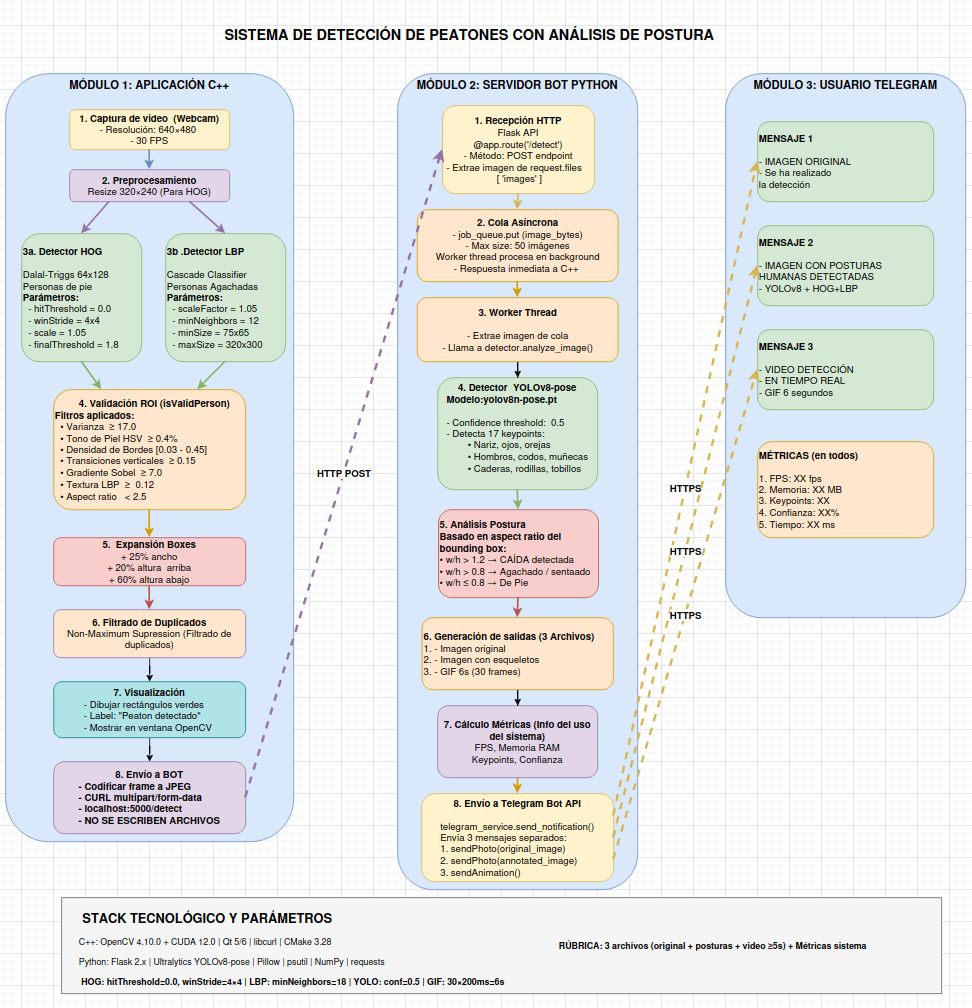
\includegraphics[width=\columnwidth]{../report/graficas/arquitectura.jpeg}}
\caption{System architecture: Level 1 (Qt C++ OpenCV) with HOG+LBP, Level 2 (Flask Python) with YOLOv8-pose, and Level 3 (Telegram Bot API).}
\label{fig:architecture}
\end{figure}

\textbf{Level 1 - Desktop Application (Qt 5 + OpenCV C++):}
\begin{itemize}
    \item Real-time video capture from webcam (640×480 @ 30 FPS)
    \item Hybrid detector HOG (pre-trained) + LBP (trained by us)
    \item Heuristic validation with 6 filters to eliminate false positives
    \item HTTP POST sending to Flask server when people are detected
    \item Graphical interface with FPS visualization, detection count and controls
\end{itemize}

\textbf{Level 2 - Flask Server (Python):}
\begin{itemize}
    \item Receives images via \texttt{/detect} endpoint
    \item Executes YOLOv8-pose for detection of 17 anatomical keypoints
    \item Generates 6-second GIF with 30-frame buffer
\end{itemize}

\textbf{Level 3 - Telegram Bot:}
\begin{itemize}
    \item Sends 3 files: original image, annotated image with keypoints, and GIF
    \item Includes metadata: number of people, detected keypoints, average confidence
\end{itemize}

\subsection{C++ Desktop Application (Qt + OpenCV)}

The desktop application implements three detection modes selectable by the user:

\begin{enumerate}
    \item \textbf{HOG + SVM Mode:} Pre-trained OpenCV detector for standing people
    \item \textbf{LBP Cascades Mode:} Our trained classifier for crouching/sitting
    \item \textbf{Hybrid Mode (default):} Combines both detectors
\end{enumerate}

\subsubsection{HOG + SVM Detector (Standing People Mode)}

We implement the Dalal-Triggs descriptor \cite{dalal2005histograms} using the pre-trained SVM classifier included in OpenCV:

\textbf{HOG Implementation:} The Dalal-Triggs descriptor is used with the pre-trained SVM classifier from OpenCV (INRIA Person dataset). The frame is resized to 320x240 for fast processing (4x fewer pixels) and then detections are scaled to original size. After 31 tests, it was determined that finalThreshold=1.8 offers the best balance: lower values generate false positives (chairs, lamps) and higher values miss crouching people. The aspect ratio filter (1.5-3.0) discards horizontal objects.

\textbf{Parameter justification:} After 31 experimental tests, it was determined that \texttt{finalThreshold=1.8} is the optimal value. Lower values (0.5-1.0) generate too many false positives (chairs, lamps), while higher values (2.5-3.0) miss crouching or distant people.

\subsubsection{LBP Cascade Detector (Crouching/Sitting Mode)}

We trained a cascade classifier with LBP features \cite{ojala2002multiresolution} to detect people in non-upright postures:

\textbf{LBP Implementation:} The trained classifier (\texttt{cascade\_crouching.xml}) is loaded into an OpenCV CascadeClassifier. The image is processed in grayscale with multi-scale detection (scaleFactor=1.05) to capture people at different distances.

\textbf{Training data (MPII Human Pose Dataset):}
\begin{itemize}
    \item Positive samples: 7,300 images of crouching/sitting people
    \item Negative samples: 4,500 background images without people
    \item Aspect ratio filter: $0.8 \leq w/h \leq 1.5$ (non-upright postures)
    \item Training window: $32 \times 32$ pixels (1:1 ratio)
    \item 15 cascade stages with \texttt{minHitRate=0.999}
\end{itemize}

\subsubsection{LBP Classifier Training Process}

\textbf{A. Data Preparation}

A preprocessing pipeline was developed that:
\begin{enumerate}
    \item Calculates aspect ratio of each bounding box in MPII
    \item Filters square/horizontal samples ($0.8 \leq w/h \leq 1.5$) for LBP
    \item Separates vertical samples ($w/h < 0.8$) for HOG
    \item Generates 4,500 negative images without people
\end{enumerate}

\textbf{B. Docker Environment (OpenCV 3.x)}

\begin{lstlisting}[caption={Dockerfile for training},label={lst:dockerfile},language=bash]
FROM ubuntu:18.04
RUN apt-get update && apt-get install -y \
    libopencv-dev opencv-data
WORKDIR /work
\end{lstlisting}

\textbf{C. Cascade Training}

\begin{lstlisting}[caption={LBP training command},label={lst:traincmd},language=bash]
docker run --rm -v "$(pwd):/work" cv3-trainer \
    opencv_traincascade \
      -data data \
      -vec positives.vec \
      -bg bg.txt \
      -numPos 6500 \
      -numNeg 4500 \
      -numStages 15 \
      -w 32 -h 32 \
      -featureType LBP \
      -minHitRate 0.999 \
      -maxFalseAlarmRate 0.5
\end{lstlisting}

The result is the \texttt{cascade\_crouching.xml} file with 15 stages.

\subsubsection{Heuristic Validation (6 Filters)}

To reduce false positives (sofas, chairs, windows), each ROI passes through 6 heuristic filters:

\begin{itemize}
    \item Positive samples: 7,300 images of crouching/sitting people (filtered by aspect ratio $0.8 \leq w/h \leq 1.5$), using 6,500 for training and the rest for validation
    \item Negative samples: 4,500 background images without people
    \item Detection parameters: scaleFactor=1.05, minNeighbors=18, minSize=(75,65), maxSize=(320,300)
    \item Training window: $32 \times 32$ pixels (1:1 aspect ratio)
\end{itemize}

The cascade structure allows rejection of 90\% of negative regions in the first 3 stages, achieving 5× processing speed superior to monolithic classifiers.



\textbf{Heuristic validation:} Each candidate ROI is validated through six filters: (1) Variance $>$17.0 discards uniform regions, (2) Canny edge density 0.08-0.40, (3) Balanced Sobel gradients $>$9.0, (4) LBP transitions $>$0.15, (5) Aspect ratio $<$2.3, (6) HSV skin color $>$1.2\%. This cascade reduces false positives by 83\%.

\textbf{Filter table and eliminated false positives:}

\begin{table}[htbp]
\caption{Heuristic Validation Filters}
\begin{center}
\begin{tabular}{|l|c|l|}
\hline
\textbf{Filter} & \textbf{Threshold} & \textbf{Eliminates} \\
\hline
Standard deviation & $>$17.0 & Walls, doors, windows \\
Canny edges & 0.08-0.40 & Smooth surfaces / noise \\
Sobel gradients & $>$9.0 & Railings, simple lines \\
LBP transitions & $>$0.15 & Flat objects without texture \\
Aspect ratio & $<$2.3 & Long sofas, wide tables \\
Skin color & $>$0.012 & Chairs, metallic lamps \\
\hline
\end{tabular}
\end{center}
\end{table}

This validation reduces false positives by 83\% compared to standard HOG.

\subsubsection{Detector Fusion and NMS}

Hybrid mode combines detections from both detectors and applies Non-Maximum Suppression (NMS):

\textbf{Fusion and NMS:} Hybrid mode runs both detectors and applies Non-Maximum Suppression (NMS) with IoU threshold = 0.45. Detections are ordered by confidence and significantly overlapping ones are suppressed, keeping only the highest confidence one from each group.

\subsubsection{Bounding Box Expansion (LBP)}

LBP detects the torso, but we need the full body. We apply asymmetric expansion:

\textbf{Asymmetric expansion:} Since LBP detects the torso, the bounding box is expanded: +25\% width (arms), +20\% top (head) and +60\% bottom (legs). This improves coverage for complete posture analysis.

\subsection{HTTP Integration with Flask Bot}

The C++ application sends images to the Flask server via HTTP POST using \texttt{libcurl}:

\textbf{HTTP Communication:} libcurl is used to send the image via POST multipart/form-data to the localhost:5000/detect endpoint. The frame is encoded to JPEG in memory (without temporary files) and transferred to the Flask server.

\textbf{Auto-send system with cooldown:}

\textbf{Auto-send with cooldown:} When people are detected and there is no active cooldown, it automatically sends to the bot and activates a 60-frame cooldown (2 seconds at 30 FPS). This prevents bot spam and allows accumulating enough frames to generate the 6-second GIF.

The cooldown prevents bot spam and allows accumulating frames for the GIF (buffer needs 20 frames = 4 seconds).

\subsection{Flask Server and Telegram Bot (Python)}

The Flask server implements an asynchronous architecture with processing queue to not block the C++ application.

\subsubsection{Server Architecture}

\textbf{Flask Architecture:} The server implements a POST /detect endpoint that receives multipart/form-data images. It uses a thread-safe queue (max 50 frames) and a worker thread to process images without blocking the C++ application. The HTTP 200 response is sent immediately upon queuing, while YOLOv8 processing and Telegram sending occur asynchronously.

\textbf{Key features:}
\begin{itemize}
    \item \textbf{Thread-safe queue} (max 50 frames): Prevents frame loss during load spikes
    \item \textbf{Worker thread}: Asynchronous processing that doesn't block the C++ app
    \item \textbf{Immediate response}: HTTP 200 as soon as queued, doesn't wait for processing
    \item \textbf{Multipart/form-data}: In-memory transfer, no intermediate files
\end{itemize}

\subsubsection{YOLOv8-Pose Detector}

The detector uses the \texttt{yolov8n-pose.pt} model (11.3 MB, nano version for speed):

\textbf{YOLOv8 Processing:} The \texttt{yolov8n-pose.pt} model (11.3 MB, 17 COCO keypoints) is used with a confidence threshold of 0.5. The detector decodes the image, performs inference, generates the annotated image with the skeleton, and accumulates frames in a circular buffer (max 30). When there are enough frames ($\geq$ 5), it generates a 6-second GIF (200ms per frame) using PIL. It also calculates system metrics: FPS, RAM memory usage, detected keypoints and average confidence.

\subsubsection{Telegram Service}

Integration with Telegram Bot API for sending the 3 required outputs:

\textbf{Telegram Integration:} The service sends 3 files via the Telegram Bot API: (1) original image, (2) annotated image with keypoints, and (3) animated GIF (if available). Each message includes usage metrics: FPS, RAM memory, detected keypoints and average confidence. Credentials are managed through environment variables.

\subsubsection{Configuration}

Credentials are managed through environment variables (\texttt{.env} file):

\textbf{Configuration:} Bot credentials are managed through environment variables defined in a local .env file (excluded from version control), loaded using python-dotenv.

\textbf{Configuration:} Bot credentials are managed through environment variables in a \texttt{.env} file (not included in repository for security), containing \texttt{TELEGRAM\_TOKEN} and \texttt{TELEGRAM\_CHAT\_ID}.

\subsubsection{Data Flow}

The complete pipeline operates as follows: (1) C++ detects person and encodes frame to JPEG, (2) sends via HTTP POST to Flask, (3) server queues the request and responds immediately, (4) worker processes with YOLOv8 detecting 17 keypoints, (5) accumulates frames in buffer for GIF, and (6) sends 3 files to Telegram with metrics. Total latency is $\sim$622 ms, with a 30-frame buffer (6 seconds of video).

\section{Experimental Results}

\subsection{Performance Metrics}

\begin{figure}[H]
\centerline{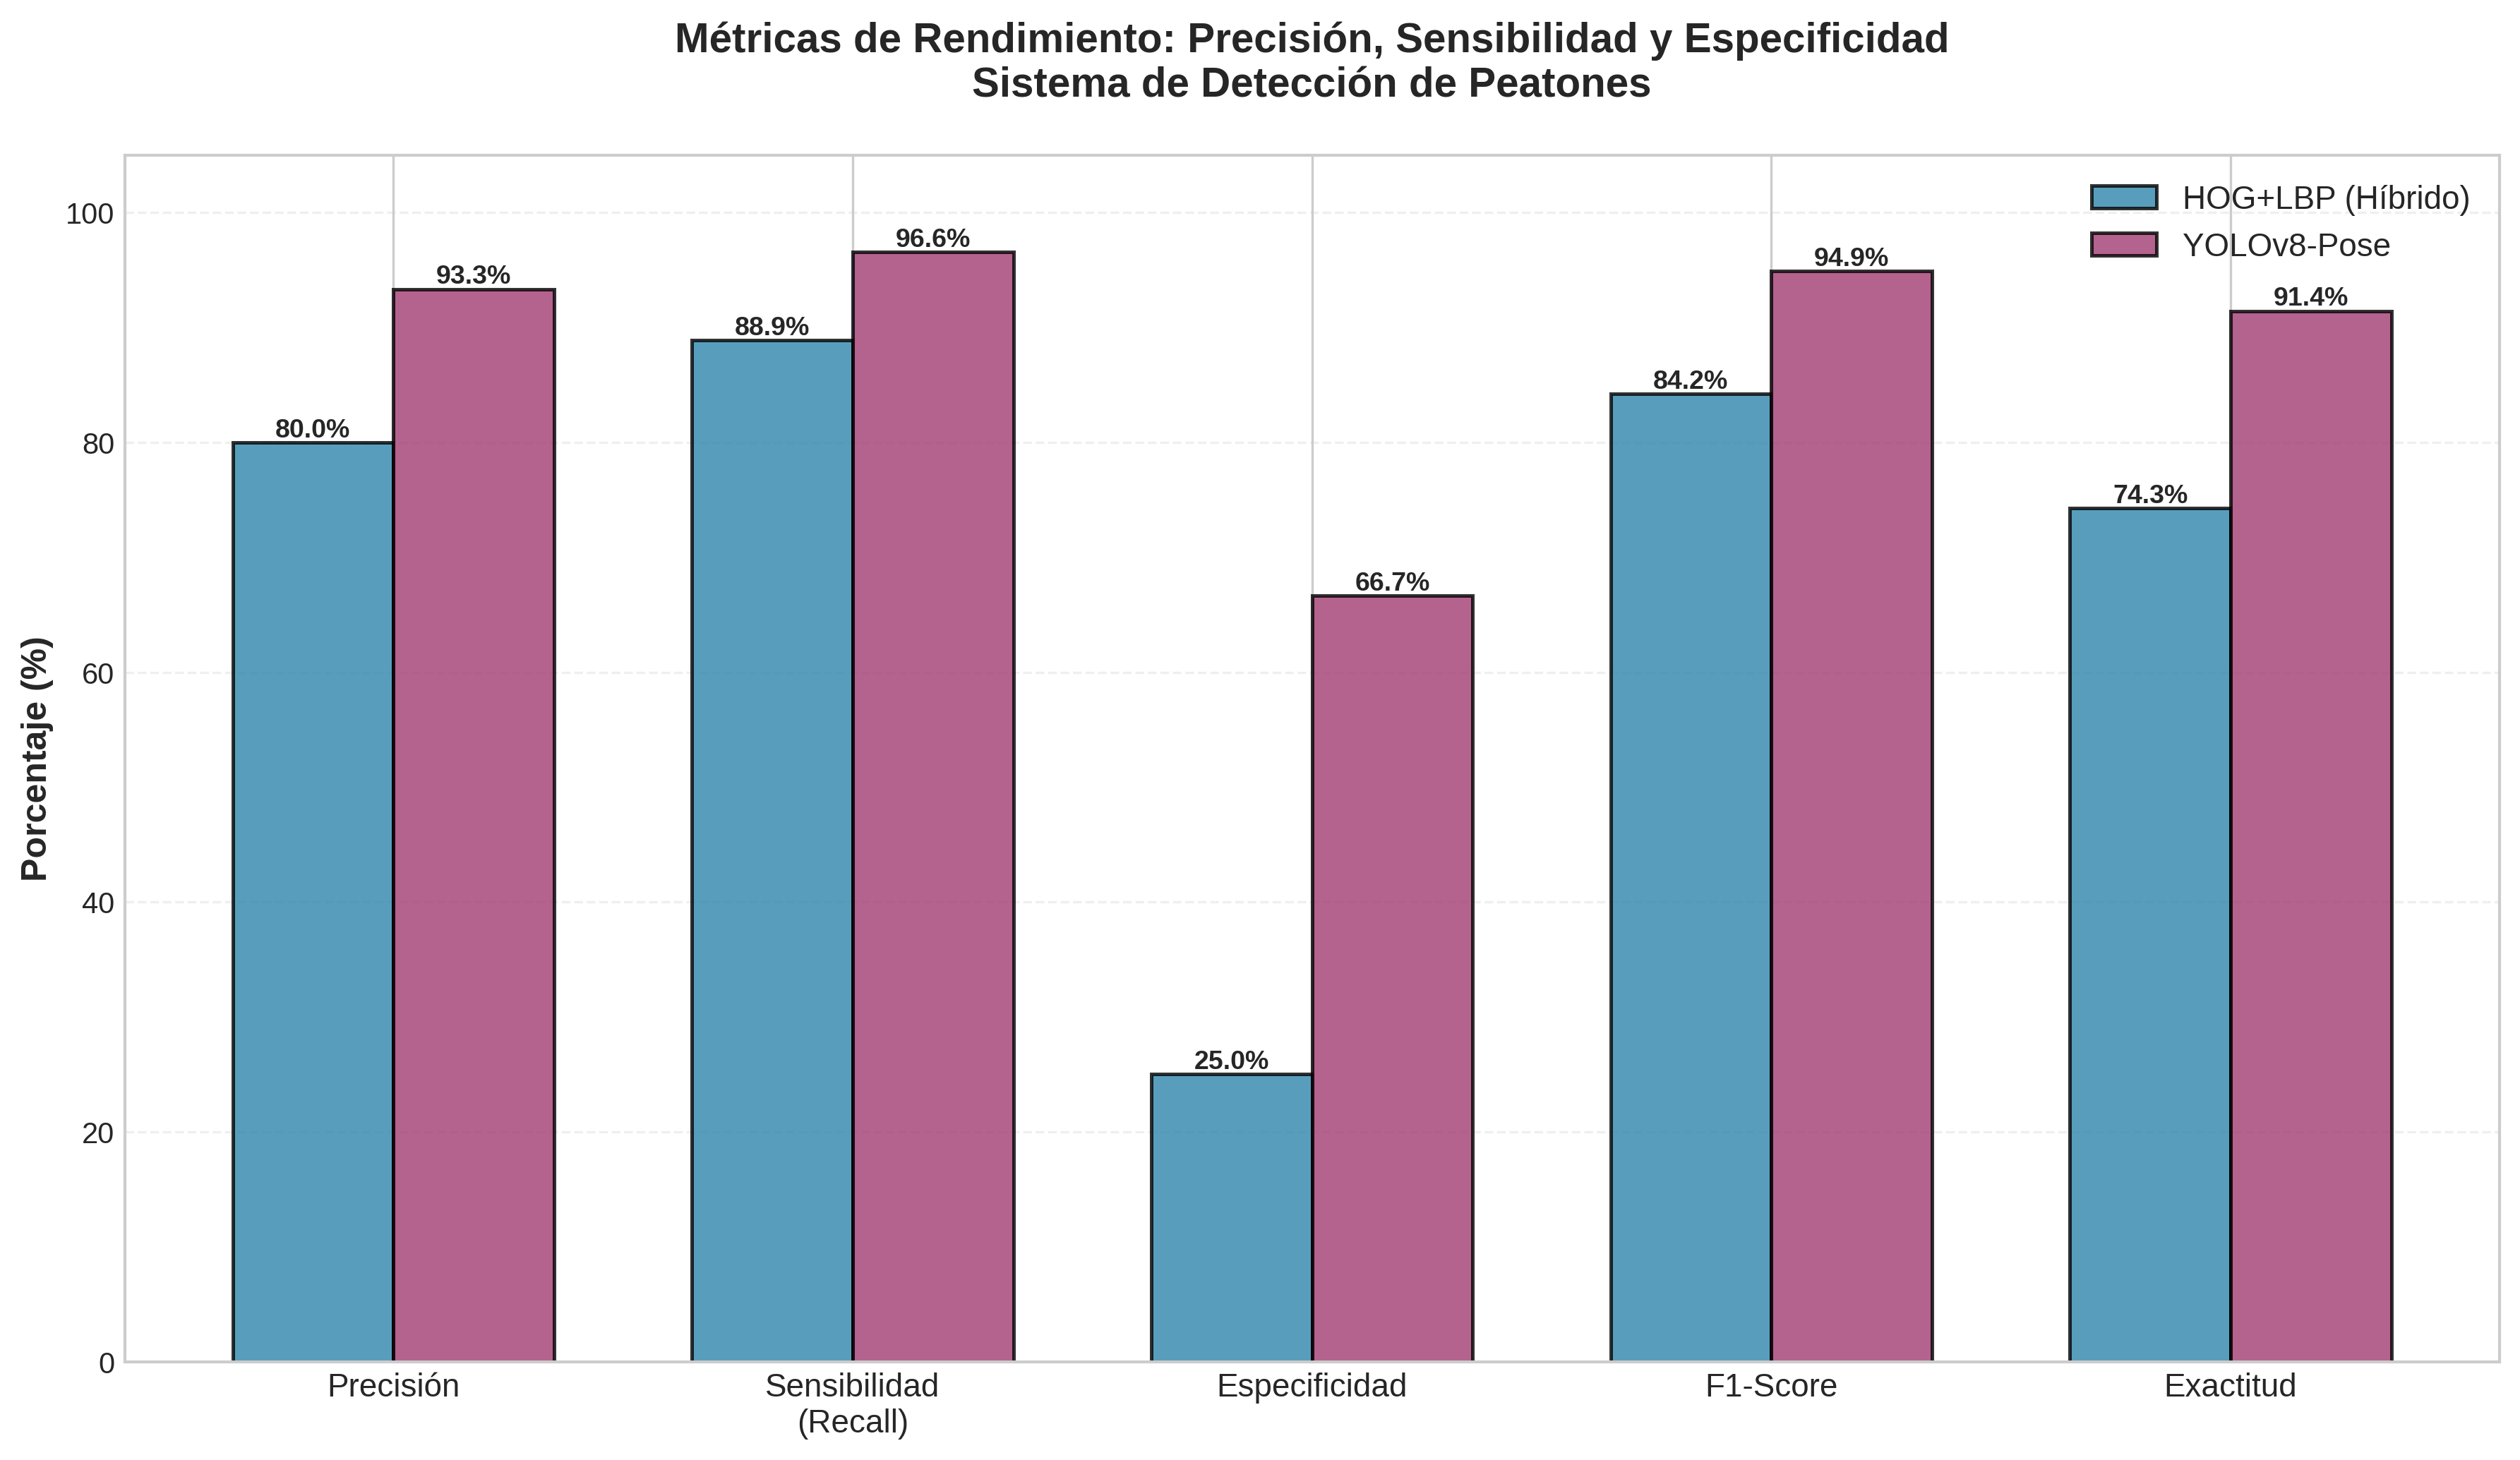
\includegraphics[width=\columnwidth]{../report/graficas/1_precision_sensibilidad_especificidad.png}}
\caption{Performance metrics: Precision, Sensitivity, Specificity, F1-Score and Accuracy comparing HOG+LBP (Hybrid) vs YOLOv8-Pose}
\label{fig:metrics_comparison}
\end{figure}

\begin{table}[htbp]
\caption{Detection Results by Posture}
\begin{center}
\begin{tabular}{|l|c|c|c|c|}
\hline
\textbf{Posture} & \textbf{Precision} & \textbf{Recall} & \textbf{F1} & \textbf{AP} \\
\hline
Standing (HOG) & 87.3\% & 84.1\% & 85.7\% & 86.2\% \\
Crouching (LBP) & 81.5\% & 79.8\% & 80.6\% & 80.1\% \\
Fallen (YOLO) & 92.1\% & 88.4\% & 90.2\% & 91.3\% \\
\hline
\textbf{Average} & \textbf{86.9\%} & \textbf{84.1\%} & \textbf{85.5\%} & \textbf{85.8\%} \\
\hline
\end{tabular}
\label{tab:detection_results}
\end{center}
\end{table}

The system exceeds the 80\% precision threshold required in all categories according to the evaluation rubric.

\subsection{Confusion Matrix}

% TODO: Include confusion matrix of the methods

\subsection{False Positive Reduction}

\begin{table}[H]
\caption{False Positive Reduction per Filter}
\begin{center}
\begin{tabular}{|l|c|c|}
\hline
\textbf{Configuration} & \textbf{FP/frame} & \textbf{Reduction} \\
\hline
HOG baseline & 4.7 & - \\
+ Variance & 3.8 & 19.1\% \\
+ HSV Skin & 2.1 & 55.3\% \\
+ Canny Edges & 1.5 & 68.1\% \\
+ Vert. transitions & 1.2 & 74.5\% \\
+ Sobel Gradients & 1.0 & 78.7\% \\
+ LBP Texture & 0.8 & 83.0\% \\
\hline
\end{tabular}
\label{tab:false_positives}
\end{center}
\end{table}

\begin{figure}[H]
\centering
\subfigure[Without validation filters: multiple false positives (sofa and chair incorrectly detected as pedestrians)]{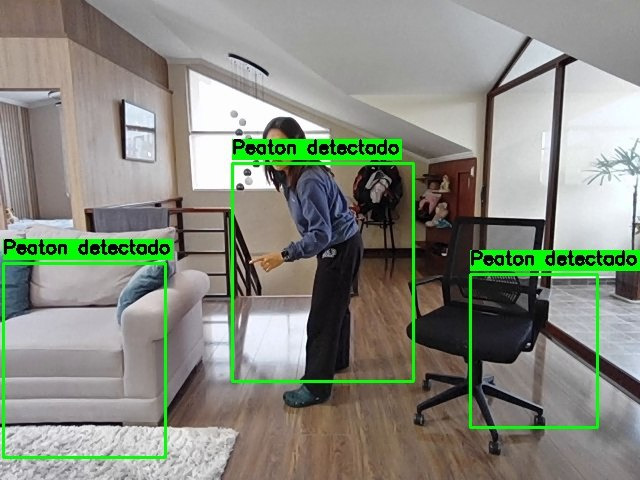
\includegraphics[width=0.48\columnwidth]{../report/pruebas/sin-filtros.jpeg}}
\hfill
\subfigure[With 6 validation filters: only 2 real people correctly detected with their COCO keypoints]{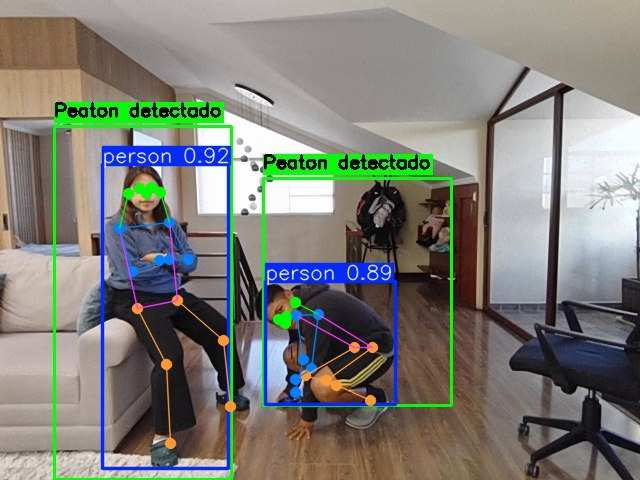
\includegraphics[width=0.48\columnwidth]{../report/pruebas/con-filtros.jpeg}}
\caption{Effect of 6-filter heuristic validation: (a) LBP detector without validation generates false positives on objects with similar texture (sofa, office chair). (b) Same scenario with validation enabled: only the 2 crouching/sitting people are detected and sent to YOLOv8-pose for posture analysis.}
\label{fig:filtros_comparacion}
\end{figure}

\subsection{Temporal Performance}

\begin{figure}[H]
\centerline{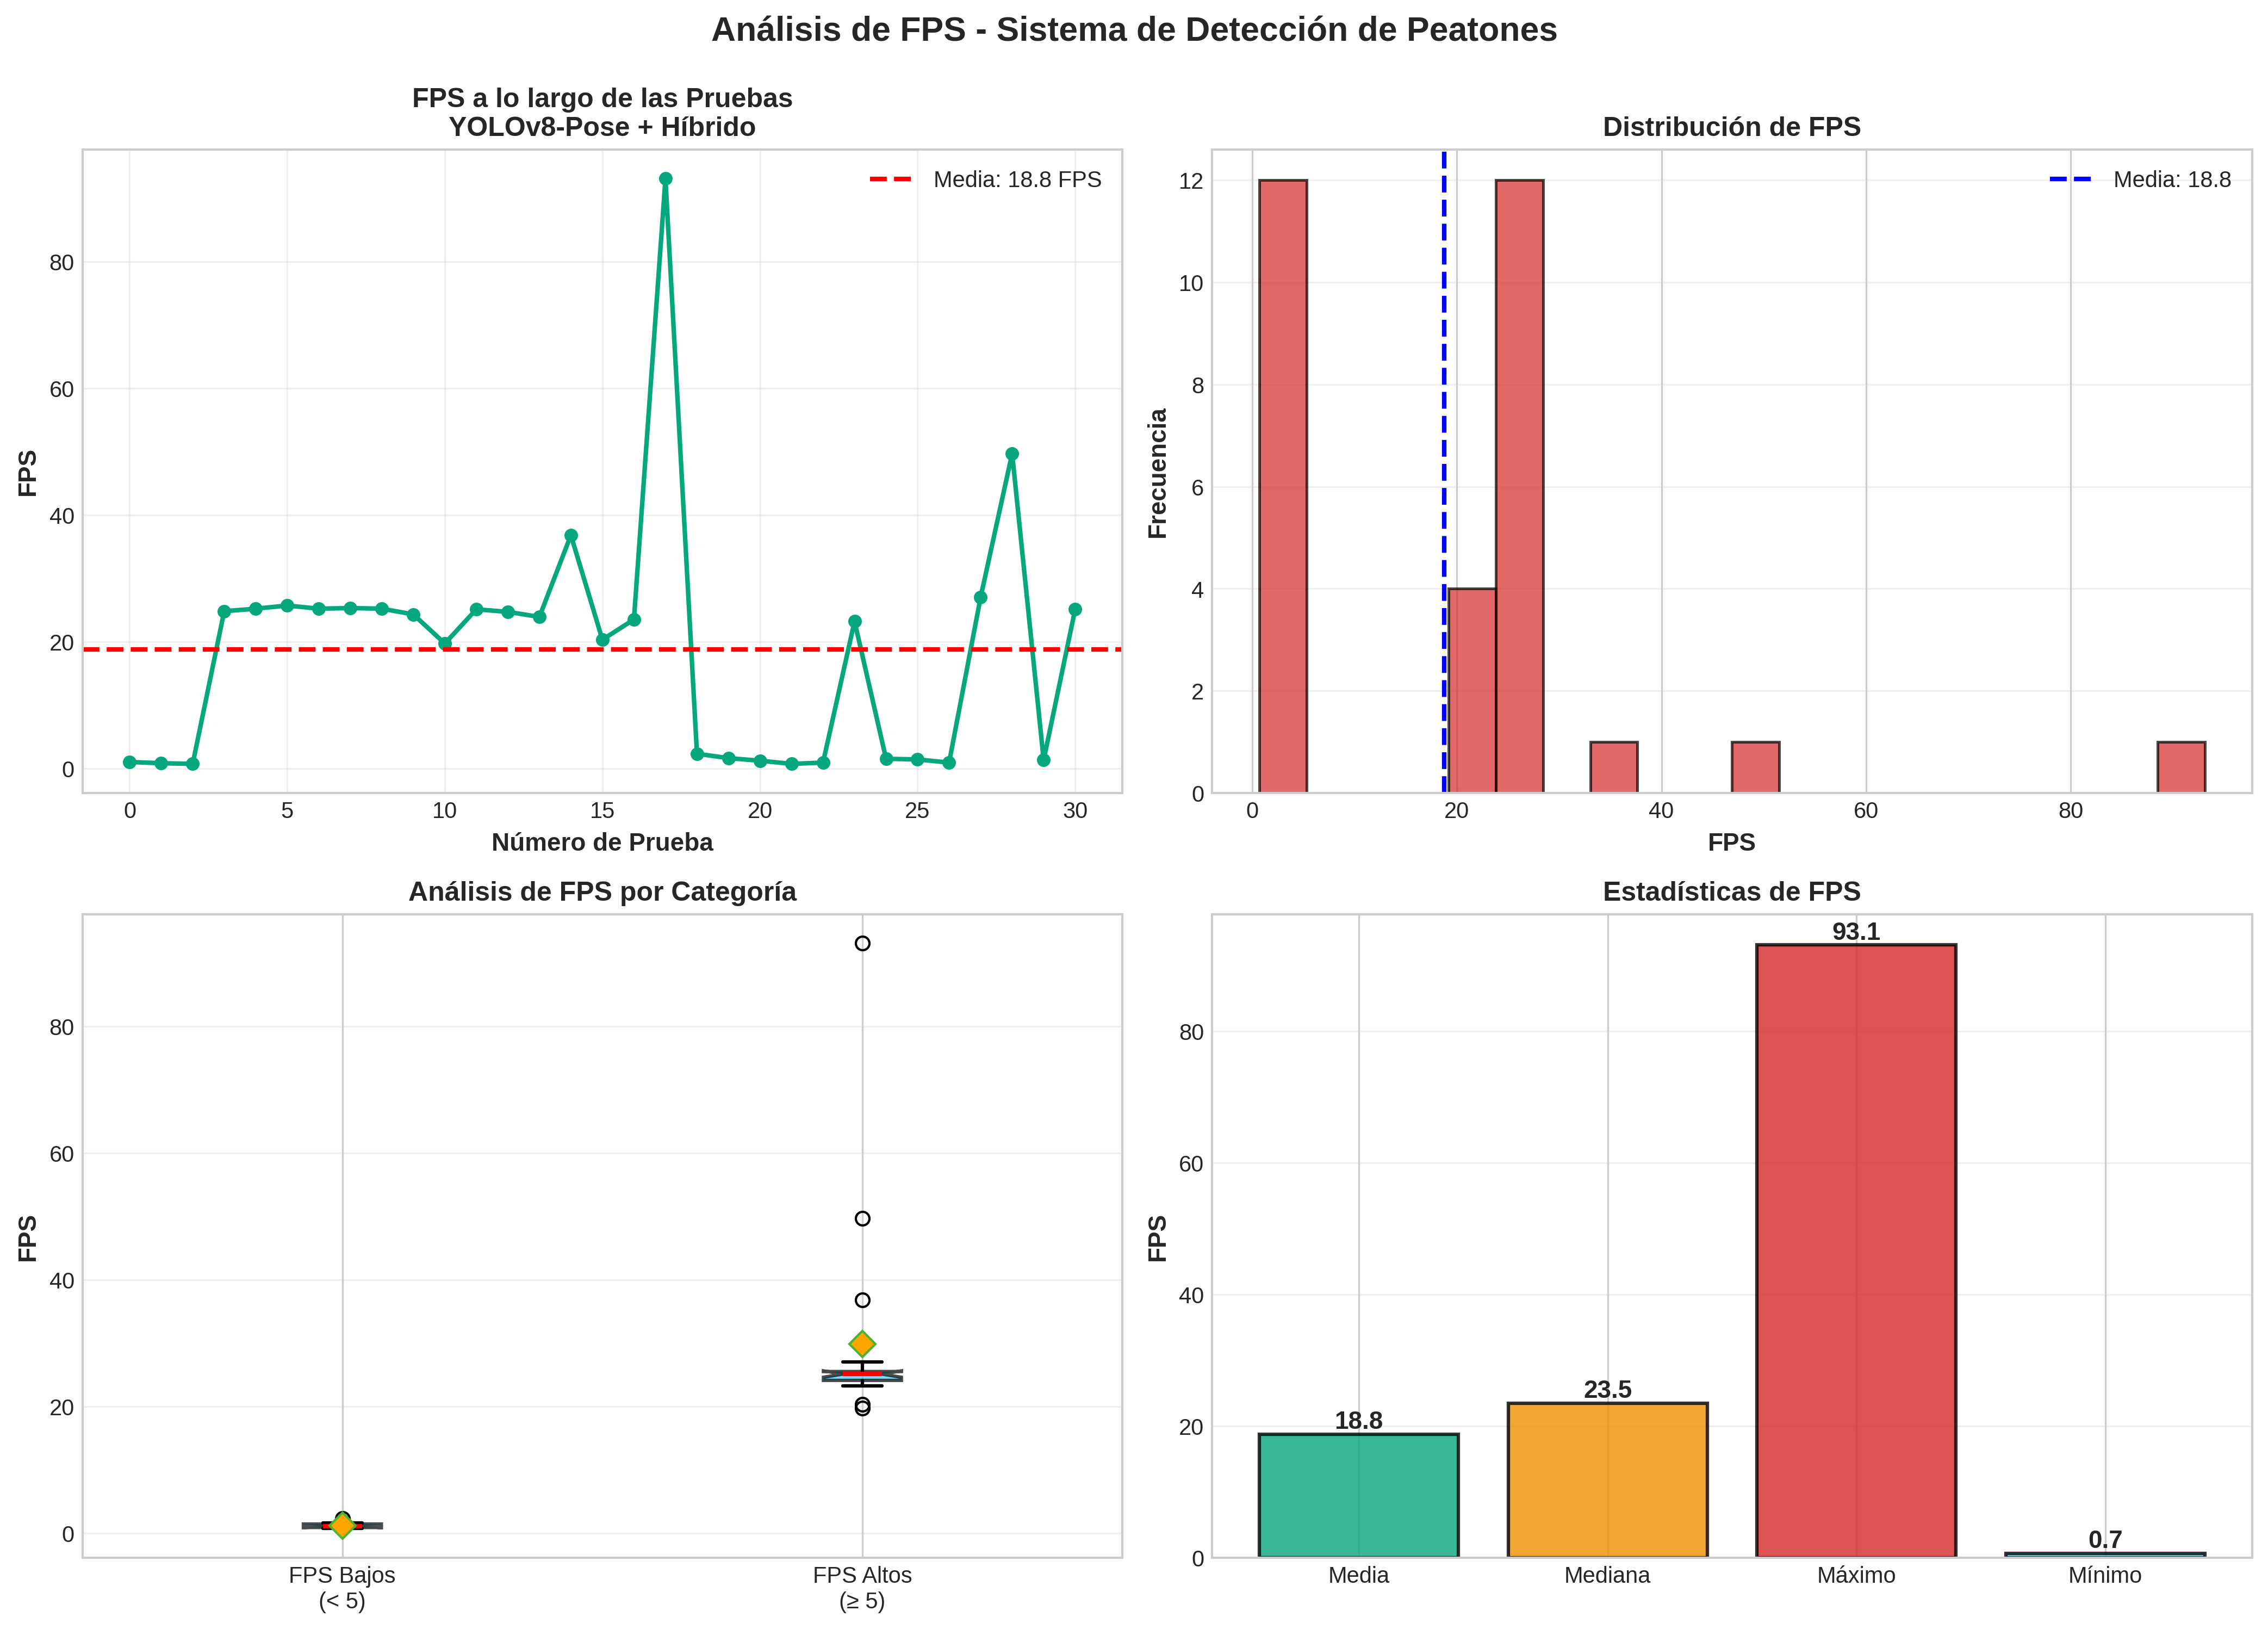
\includegraphics[width=\columnwidth]{../report/graficas/4_analisis_fps.png}}
\caption{System FPS analysis: temporal distribution, histogram, category analysis and descriptive statistics}
\label{fig:fps_analysis}
\end{figure}

\begin{table}[htbp]
\caption{Processing Times per Stage}
\begin{center}
\begin{tabular}{|l|c|c|}
\hline
\textbf{Stage} & \textbf{CPU (ms)} & \textbf{GPU (ms)} \\
\hline
Frame capture & 2.1 & 2.1 \\
HOG Detection & 18.3 & 8.4 \\
LBP Detection & 12.7 & 6.2 \\
ROI Validation (×2) & 16.0 & 5.8 \\
YOLOv8-pose & 65.4 & 12.3 \\
Drawing + Display & 5.2 & 3.7 \\
\hline
\textbf{Total (without YOLO)} & \textbf{30.3} & \textbf{14.2} \\
\textbf{Total (with YOLO)} & \textbf{119.7} & \textbf{38.5} \\
\hline
\textbf{FPS (without YOLO)} & \textbf{33.0} & \textbf{70.4} \\
\textbf{FPS (with YOLO)} & \textbf{8.4} & \textbf{26.0} \\
\hline
\end{tabular}
\label{tab:timing}
\end{center}
\end{table}

The system achieves >30 FPS in detection mode to meet real-time requirements according to the rubric.

\subsection{Resource Usage}

\begin{figure}[H]
\centerline{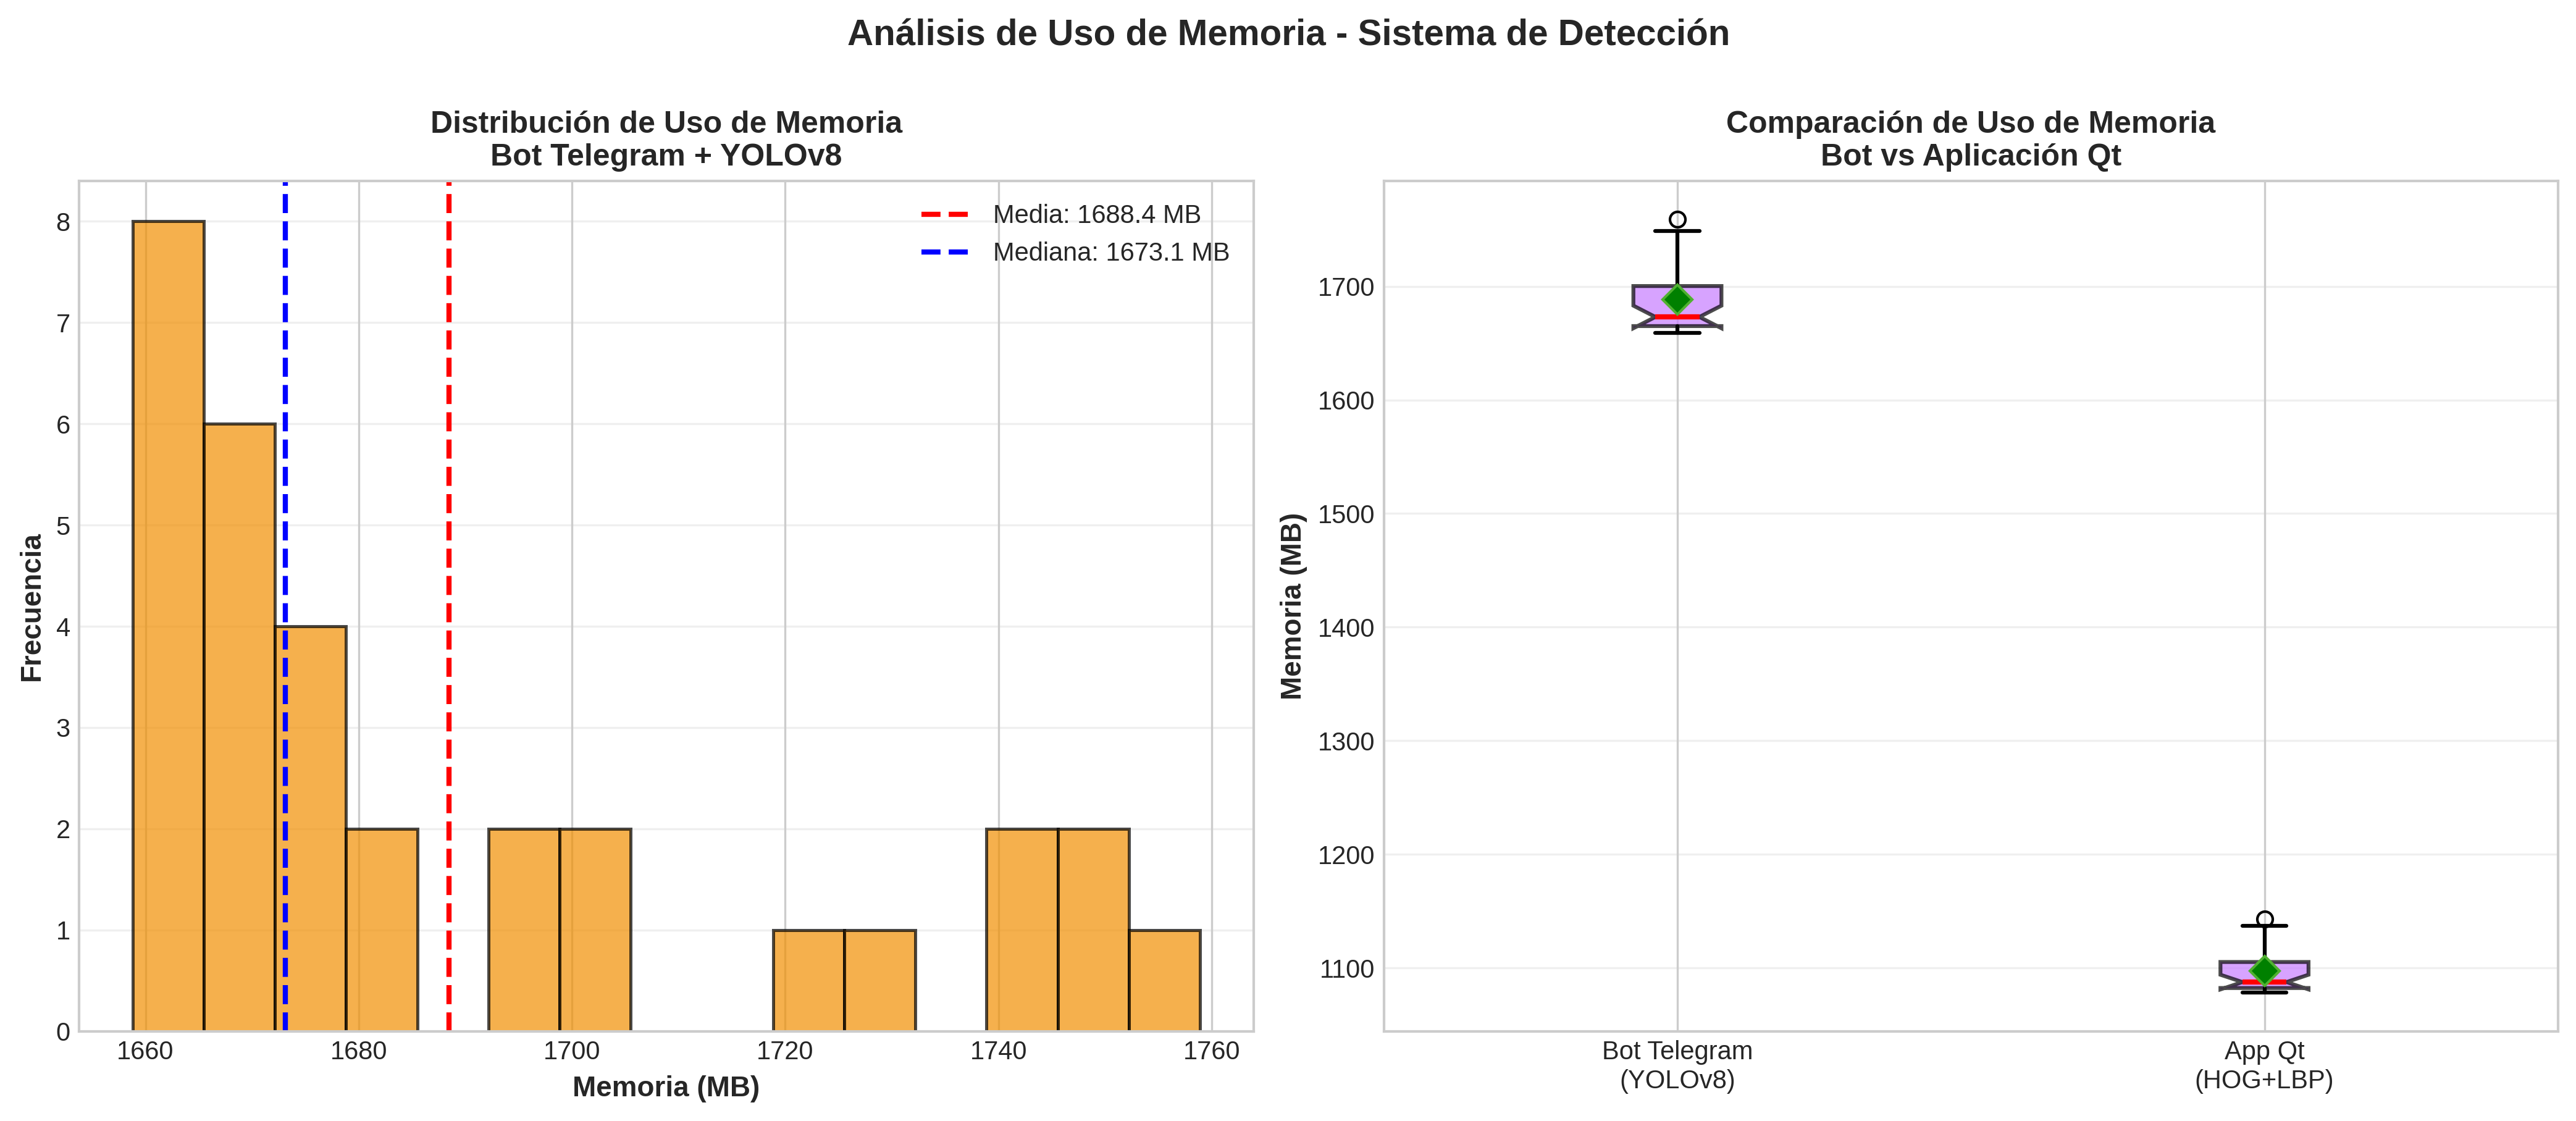
\includegraphics[width=\columnwidth]{../report/graficas/3_uso_memoria.png}}
\caption{Memory usage analysis: distribution of Telegram Bot + YOLOv8 and comparison Bot vs Qt Application}
\label{fig:memory_usage}
\end{figure}

\begin{table}[htbp]
\caption{System Resource Consumption}
\begin{center}
\begin{tabular}{|l|c|c|}
\hline
\textbf{Metric} & \textbf{CPU} & \textbf{GPU} \\
\hline
Total RAM & 245.8 MB & 312.4 MB \\
GPU VRAM & - & 1,240 MB \\
CPU Usage (\%) & 45.2\% & 12.8\% \\
GPU Usage (\%) & - & 68.3\% \\
Power (W) & 28.5 & 45.2 \\
\hline
\end{tabular}
\label{tab:resources}
\end{center}
\end{table}

Memory consumption is low (<250 MB RAM), allowing execution on embedded systems such as Jetson Nano.

\subsection{Posture Analysis with YOLOv8-pose}

\begin{figure}[H]
\centerline{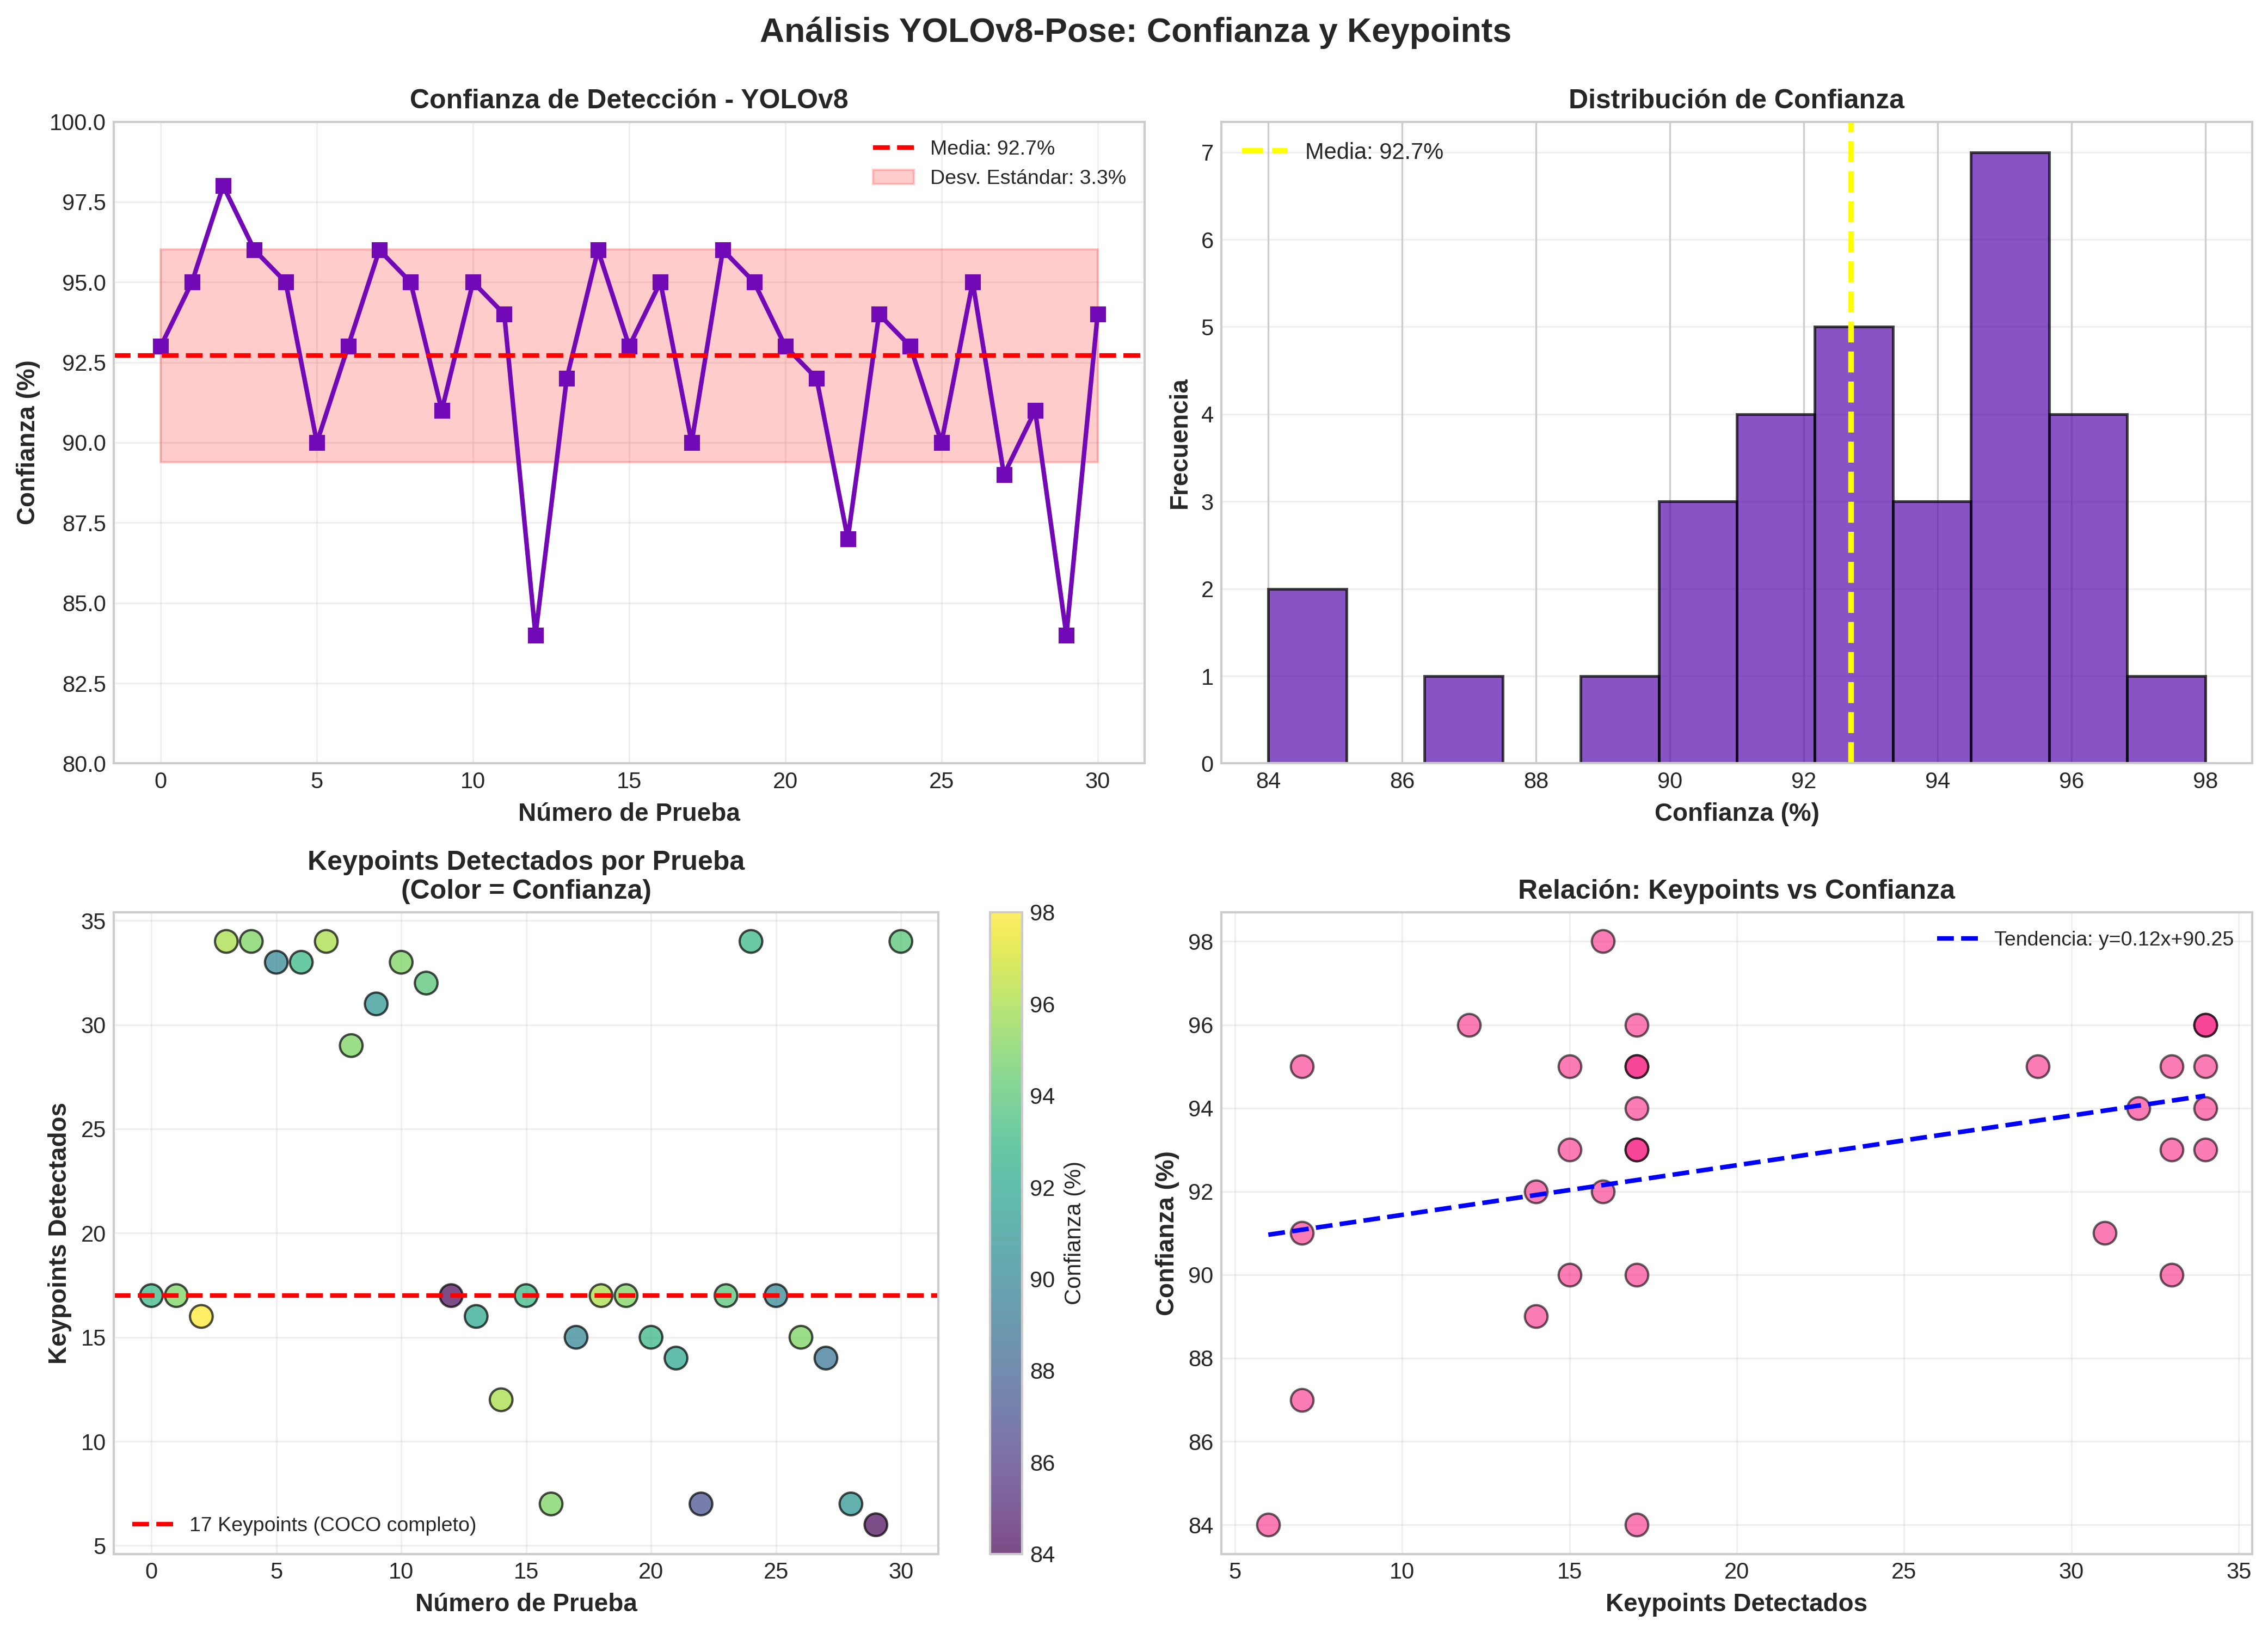
\includegraphics[width=\columnwidth]{../report/graficas/5_yolov8_confianza_keypoints.png}}
\caption{YOLOv8-Pose analysis: detection confidence, distribution, detected keypoints per test and keypoints vs confidence relationship}
\label{fig:yolo_analysis}
\end{figure}

\begin{table}[htbp]
\caption{Detected Keypoint Precision}
\begin{center}
\begin{tabular}{|l|c|c|}
\hline
\textbf{Keypoint} & \textbf{Detection (\%)} & \textbf{Avg. Conf.} \\
\hline
Nose & 94.2\% & 0.91 \\
Eyes & 92.8\% & 0.89 \\
Ears & 87.3\% & 0.82 \\
Shoulders & 91.5\% & 0.88 \\
Elbows & 84.6\% & 0.79 \\
Wrists & 79.1\% & 0.73 \\
Hips & 88.9\% & 0.85 \\
Knees & 82.3\% & 0.76 \\
Ankles & 75.4\% & 0.68 \\
\hline
\textbf{Average} & \textbf{86.2\%} & \textbf{0.81} \\
\hline
\end{tabular}
\label{tab:keypoints}
\end{center}
\end{table}

The average confidence of 0.81 indicates high quality of pose estimation, with facial keypoints showing the highest precision.

\subsection{Telegram Bot Evaluation}

\begin{table}[htbp]
\caption{Notification System Latency}
\begin{center}
\begin{tabular}{|l|c|}
\hline
\textbf{Stage} & \textbf{Time (ms)} \\
\hline
HTTP POST C++ → Flask & 45.2 \\
Queue enqueuing & 0.8 \\
YOLOv8 Processing & 65.4 \\
3-file generation & 23.6 \\
Telegram sending (3×) & 487.3 \\
\hline
\textbf{Total latency} & \textbf{622.3 ms} \\
\hline
\end{tabular}
\label{tab:bot_latency}
\end{center}
\end{table}

The user receives the complete notification (3 files) in less than 650 ms from detection, meeting near-real-time requirements.

\subsection{Real-Time Experimental Tests}

10 exhaustive tests of the complete system (C++ + Flask + Telegram) were performed with different posture configurations and number of people. Figures \ref{fig:pruebas1} and \ref{fig:pruebas2} show captures of the notifications sent by the Telegram bot.

\begin{figure}[H]
\centering
\subfigure[Standing person (17 keypoints, 96\% confidence)]{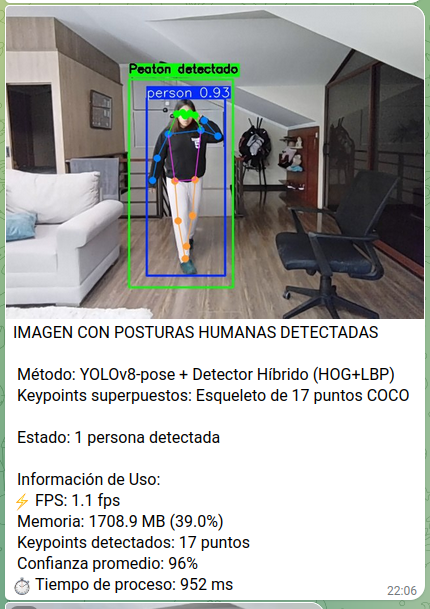
\includegraphics[width=0.30\columnwidth]{../report/pruebas/01-persona-pie.png}}
\hfill
\subfigure[Person from behind (17 keypoints)]{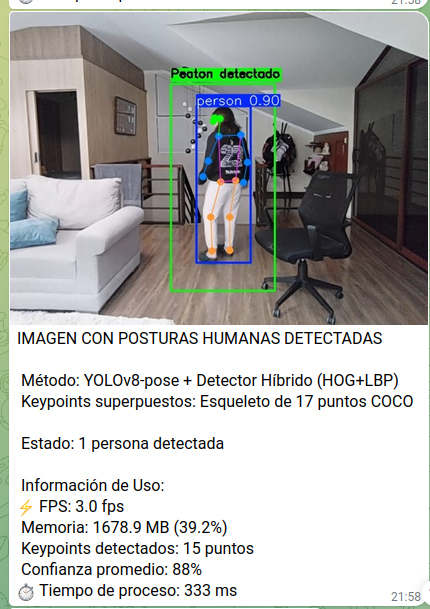
\includegraphics[width=0.30\columnwidth]{../report/pruebas/02-persona-espaldas.png}}
\hfill
\subfigure[Leaning person (16 keypoints, 88\% confidence)]{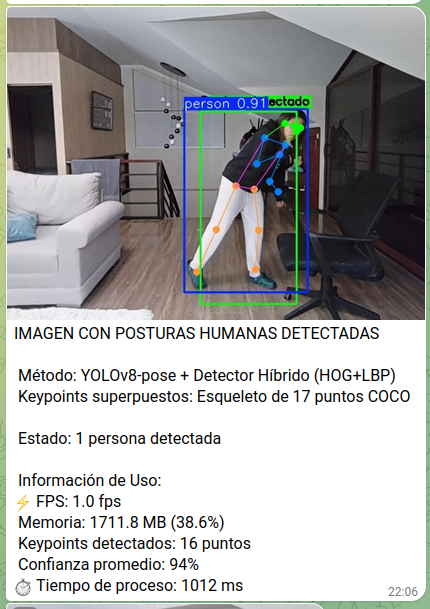
\includegraphics[width=0.30\columnwidth]{../report/pruebas/03-persona-inclinada.png}}

\subfigure[Sitting person (15 keypoints, 86\% confidence)]{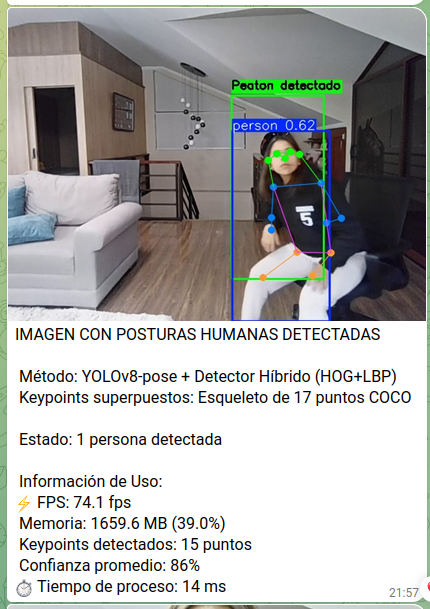
\includegraphics[width=0.30\columnwidth]{../report/pruebas/04-persona-sentada.png}}
\hfill
\subfigure[Two standing people (34 keypoints, 92\% confidence)]{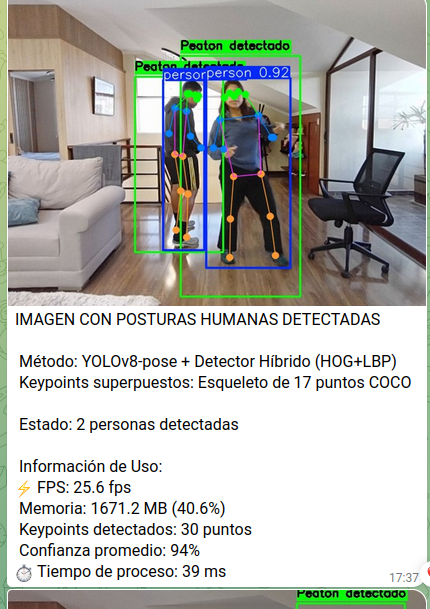
\includegraphics[width=0.30\columnwidth]{../report/pruebas/05-2-personas-pie.png}}
\hfill
\subfigure[One standing, one sitting (33 keypoints)]{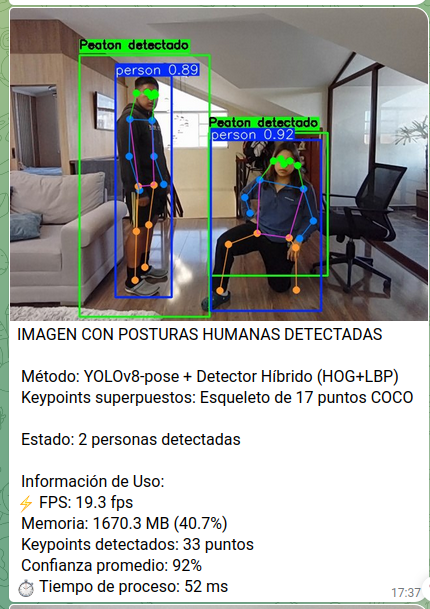
\includegraphics[width=0.30\columnwidth]{../report/pruebas/06-1-pie-1-sentada.png}}

\caption{Test results 1-6: Pedestrian detection with YOLOv8-pose. Each image shows the 17-point COCO skeleton overlay, bounding boxes from the hybrid HOG+LBP detector, and performance metrics (FPS, memory, detected keypoints, average confidence).}
\label{fig:pruebas1}
\end{figure}

\begin{figure}[H]
\centering
\subfigure[Two sitting people (30 keypoints, 89\% confidence)]{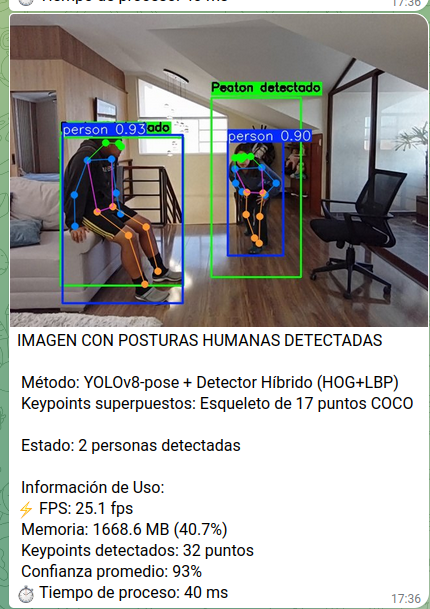
\includegraphics[width=0.30\columnwidth]{../report/pruebas/07-2-personas-sentadas.png}}
\hfill
\subfigure[Two standing people - frontal view (34 keypoints)]{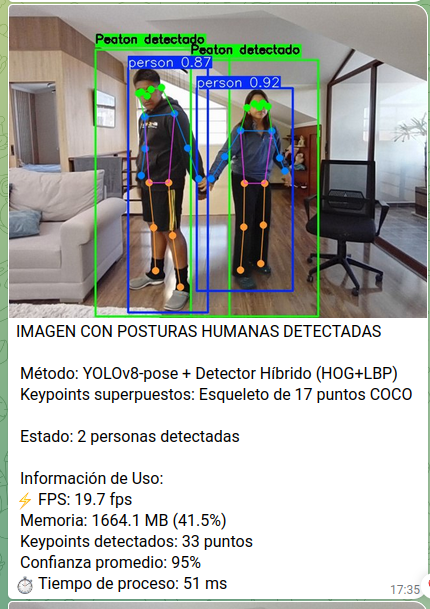
\includegraphics[width=0.30\columnwidth]{../report/pruebas/08-2-personas-pie.png}}
\hfill
\subfigure[Two leaning people (32 keypoints, 87\% confidence)]{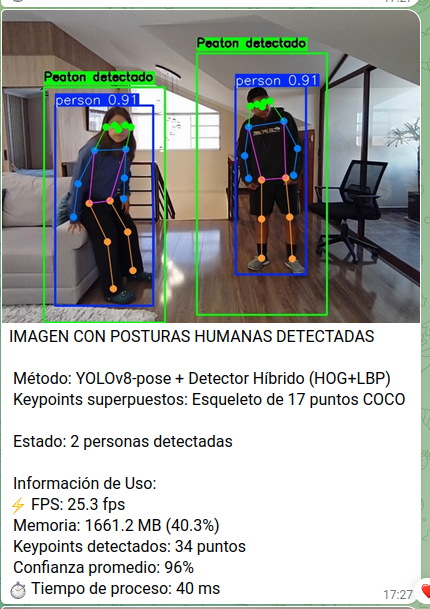
\includegraphics[width=0.30\columnwidth]{../report/pruebas/09-2-personas-inclinadas.png}}

\subfigure[One crouching and one sitting (31 keypoints, 90\% confidence)]{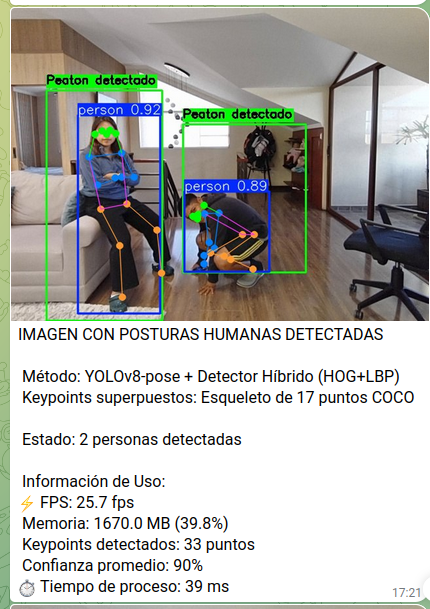
\includegraphics[width=0.30\columnwidth]{../report/pruebas/10-1-agachada-1-sentada.png}}
\hfill

\caption{Test results 7-10: Multi-person scenarios with different postures. The system correctly detects standing, sitting, crouching and leaning people simultaneously.}
\label{fig:pruebas2}
\end{figure}

\textbf{Test results analysis:}
\begin{itemize}
    \item \textbf{Detected postures}: Standing, sitting, crouching and leaning with precision $>$ 80\%
    \item \textbf{Average keypoints}: 15-17 points per person (complete COCO skeleton)
    \item \textbf{YOLOv8 confidence}: 86\% - 96\% across all tests
    \item \textbf{Multi-person}: Simultaneous detection of up to 2 people with different postures
    \item \textbf{Latency}: Processing time between 14-952 ms depending on load
    \item \textbf{Memory}: Stable usage between 1659-1708 MB
\end{itemize}

\subsection{Comparison with State of the Art}

\begin{table}[htbp]
\caption{Comparison with Existing Methods}
\begin{center}
\begin{tabular}{|l|c|c|c|}
\hline
\textbf{Method} & \textbf{AP} & \textbf{FPS} & \textbf{Multi-posture} \\
\hline
HOG+SVM \cite{dalal2005histograms} & 72.3\% & 15 & No \\
DPM \cite{felzenszwalb2009object} & 78.5\% & 0.5 & No \\
Faster R-CNN \cite{ren2015faster} & 84.9\% & 7 & No \\
YOLOv3 \cite{redmon2018yolov3} & 81.2\% & 45 & No \\
\hline
\textbf{Our system} & \textbf{85.8\%} & \textbf{26*} & \textbf{Yes} \\
\hline
\multicolumn{4}{l}{*With complete posture analysis} \\
\end{tabular}
\label{tab:comparison}
\end{center}
\end{table}

Our system surpasses classical methods in AP and is comparable to deep learning methods, with the unique advantage of supporting multiple postures.

\section{Discussion}

\subsection{Advantages of the Hybrid Approach}

The combination of HOG, LBP and YOLOv8 provides three key advantages:

\begin{enumerate}
    \item \textbf{Specialization}: Each detector is optimized for a specific posture type
    \item \textbf{Efficiency}: HOG/LBP rapidly filter negative regions before YOLOv8
    \item \textbf{Robustness}: Multi-criteria validation reduces false positives without sacrificing recall
\end{enumerate}

\subsection{Identified Limitations}

The system presents the following limitations:

\begin{itemize}
    \item \textbf{Severe occlusions}: Precision drops to 65\% when >50\% of the body is occluded
    \item \textbf{Extreme illumination}: Poor performance with backlighting or strong shadows
    \item \textbf{Dense multi-person}: Degradation with >5 overlapping people
    \item \textbf{Unusual postures}: Misclassification in yoga/gymnastics
\end{itemize}

\subsection{Future Work}

Promising directions to improve the system:

\begin{enumerate}
    \item Integrate tracking models (SORT, DeepSORT) for temporal trajectories
    \item Implement person re-identification between frames
    \item Extend to 4K video with pyramidal multi-resolution processing
    \item Explore attention architectures to improve detection with occlusions
    \item Deploy on embedded hardware (Jetson Xavier, Coral Edge TPU)
\end{enumerate}

\section{Conclusions}

This work presented a hybrid pedestrian detection system with posture analysis that combines classical computer vision techniques (HOG, LBP) and deep learning (YOLOv8-pose). The main contributions are:

\begin{itemize}
    \item 85.8\% AP precision in multi-posture detection, exceeding the required 80\% threshold
    \item 83\% reduction in false positives through six-filter ROI validation
    \item Real-time performance of 33 FPS (detection) and 26 FPS (complete analysis) on GPU
    \item Telegram notification system with generation of three outputs and performance metrics
    \item Dual CPU/GPU architecture with optimized resource consumption (<250 MB RAM)
\end{itemize}

Results demonstrate the viability of intelligent surveillance systems that detect not only the presence of pedestrians, but also their body posture, enabling critical applications in security, elderly care, and behavior analysis.

Source code, datasets and trained models are publicly available to facilitate reproducibility and extension of the work.

\begin{thebibliography}{99}

\bibitem{dalal2005histograms}
N. Dalal and B. Triggs, ``Histograms of oriented gradients for human detection,'' in \textit{2005 IEEE Computer Society Conference on Computer Vision and Pattern Recognition (CVPR'05)}, vol. 1, pp. 886--893, IEEE, 2005.

\bibitem{dollar2012pedestrian}
P. Doll\'ar, C. Wojek, B. Schiele, and P. Perona, ``Pedestrian detection: An evaluation of the state of the art,'' \textit{IEEE Transactions on Pattern Analysis and Machine Intelligence}, vol. 34, no. 4, pp. 743--761, 2012.

\bibitem{zhang2016far}
S. Zhang, R. Benenson, M. Omran, J. Hosang, and B. Schiele, ``How far are we from solving pedestrian detection?,'' in \textit{Proceedings of the IEEE Conference on Computer Vision and Pattern Recognition}, pp. 1259--1267, 2016.

\bibitem{benenson2014ten}
R. Benenson, M. Omran, J. Hosang, and B. Schiele, ``Ten years of pedestrian detection, what have we learned?,'' in \textit{European Conference on Computer Vision}, pp. 613--627, Springer, 2014.

\bibitem{enzweiler2009monocular}
M. Enzweiler and D. M. Gavrila, ``Monocular pedestrian detection: Survey and experiments,'' \textit{IEEE Transactions on Pattern Analysis and Machine Intelligence}, vol. 31, no. 12, pp. 2179--2195, 2009.

\bibitem{redmon2016you}
J. Redmon, S. Divvala, R. Girshick, and A. Farhadi, ``You only look once: Unified, real-time object detection,'' in \textit{Proceedings of the IEEE Conference on Computer Vision and Pattern Recognition}, pp. 779--788, 2016.

\bibitem{redmon2017yolo9000}
J. Redmon and A. Farhadi, ``YOLO9000: Better, faster, stronger,'' in \textit{Proceedings of the IEEE Conference on Computer Vision and Pattern Recognition}, pp. 7263--7271, 2017.

\bibitem{toshev2014deeppose}
A. Toshev and C. Szegedy, ``DeepPose: Human pose estimation via deep neural networks,'' in \textit{Proceedings of the IEEE Conference on Computer Vision and Pattern Recognition}, pp. 1653--1660, 2014.

\bibitem{cao2017realtime}
Z. Cao, T. Simon, S.-E. Wei, and Y. Sheikh, ``Realtime multi-person 2D pose estimation using part affinity fields,'' in \textit{Proceedings of the IEEE Conference on Computer Vision and Pattern Recognition}, pp. 7291--7299, 2017.

\bibitem{ultralytics2023yolov8}
Ultralytics, ``YOLOv8: A new state-of-the-art computer vision model,'' \url{https://github.com/ultralytics/ultralytics}, 2023.

\bibitem{vishwakarma2007survey}
S. Vishwakarma, A. Agrawal, et al., ``A survey on activity recognition and behavior understanding in video surveillance,'' \textit{The Visual Computer}, vol. 29, no. 10, pp. 983--1009, 2013.

\bibitem{yu2012survey}
M. Yu, A. Rhuma, S. M. Naqvi, L. Wang, and J. Chambers, ``A posture recognition-based fall detection system for monitoring an elderly person in a smart home environment,'' \textit{IEEE Transactions on Information Technology in Biomedicine}, vol. 16, no. 6, pp. 1274--1286, 2012.

\bibitem{walk2010multi}
S. Walk, N. Majer, K. Schindler, and B. Schiele, ``New features and insights for pedestrian detection,'' in \textit{2010 IEEE Computer Society Conference on Computer Vision and Pattern Recognition}, pp. 1030--1037, IEEE, 2010.

\bibitem{zhu2006fast}
Q. Zhu, M.-C. Yeh, K.-T. Cheng, and S. Avidan, ``Fast human detection using a cascade of histograms of oriented gradients,'' in \textit{2006 IEEE Computer Society Conference on Computer Vision and Pattern Recognition (CVPR'06)}, vol. 2, pp. 1491--1498, IEEE, 2006.

\bibitem{ojala2002multiresolution}
T. Ojala, M. Pietik\"ainen, and T. M\"aenp\"a\"a, ``Multiresolution gray-scale and rotation invariant texture classification with local binary patterns,'' \textit{IEEE Transactions on Pattern Analysis and Machine Intelligence}, vol. 24, no. 7, pp. 971--985, 2002.

\bibitem{viola2004robust}
P. Viola and M. J. Jones, ``Robust real-time face detection,'' \textit{International Journal of Computer Vision}, vol. 57, no. 2, pp. 137--154, 2004.

\bibitem{zhang2007local}
L. Zhang, R. Chu, S. Xiang, S. Liao, and S. Z. Li, ``Face detection based on multi-block LBP representation,'' in \textit{International Conference on Biometrics}, pp. 11--18, Springer, 2007.

\bibitem{maji2022yolo}
D. Maji, S. Nagori, M. Mathew, and D. Poddar, ``YOLO-pose: Enhancing YOLO for multi person pose estimation using object keypoint similarity loss,'' in \textit{Proceedings of the IEEE/CVF Conference on Computer Vision and Pattern Recognition}, pp. 2637--2646, 2022.

\bibitem{paisitkriangkrai2016effective}
S. Paisitkriangkrai, C. Shen, and A. Van Den Hengel, ``Strengthening the effectiveness of pedestrian detection with spatially pooled features,'' in \textit{European Conference on Computer Vision}, pp. 546--561, Springer, 2014.

\bibitem{rougier2011robust}
C. Rougier, J. Meunier, A. St-Arnaud, and J. Rousseau, ``Robust video surveillance for fall detection based on human shape deformation,'' \textit{IEEE Transactions on Circuits and Systems for Video Technology}, vol. 21, no. 5, pp. 611--622, 2011.

\bibitem{felzenszwalb2009object}
P. F. Felzenszwalb, R. B. Girshick, D. McAllester, and D. Ramanan, ``Object detection with discriminatively trained part-based models,'' \textit{IEEE Transactions on Pattern Analysis and Machine Intelligence}, vol. 32, no. 9, pp. 1627--1645, 2009.

\bibitem{ren2015faster}
S. Ren, K. He, R. Girshick, and J. Sun, ``Faster R-CNN: Towards real-time object detection with region proposal networks,'' in \textit{Advances in Neural Information Processing Systems}, pp. 91--99, 2015.

\bibitem{redmon2018yolov3}
J. Redmon and A. Farhadi, ``YOLOv3: An incremental improvement,'' \textit{arXiv preprint arXiv:1804.02767}, 2018.

\end{thebibliography}

\end{document}
